\documentclass[12pt]{article}

% LuaLaTeX basics
\usepackage{fontspec}
\usepackage{amsmath}
\usepackage{mathtools}
\usepackage{unicode-math}
% Fonts (Libertine-Äquivalent, modern)
\setmainfont{Libertinus Serif}
\setsansfont{Libertinus Sans}
\setmonofont{Libertinus Mono}

% Layout & typography
\usepackage[a4paper]{geometry}
\usepackage{setspace}
\usepackage{parskip}
\usepackage{graphicx}
\usepackage{amsmath}
\usepackage{booktabs}
\usepackage{tabularx}

% Chemistry
\usepackage{chemfig}
\usepackage[modules]{chemmacros}
\usepackage{siunitx}
\chemsetup{
  modules = {
    reactions,
    spectroscopy,
    scheme
  },
  formula = mhchem
}
\usepackage{fancyhdr}
\usepackage{overcite}
\usepackage{hyperref}
\usepackage{tabulary}


\usepackage[ddmmyyyy]{datetime}
\renewcommand{\dateseparator}{.}
\usepackage{overcite}
\renewcommand\citeform[1]{[#1]}


\newcommand\textbox[1]{%
  \parbox{.333\textwidth}{#1}%
}

\pagestyle{fancy}

\cfoot{\thepage}

\lhead{Nevroz Arslan }
\rhead{\today}
\setlength{\headheight}{15pt}

\renewcommand{\thesection}{\arabic{section}.}
\renewcommand{\thesubsection}{\thesection\arabic{subsection}}
\renewcommand{\headrulewidth}{0pt}

\begin{document}

\begingroup
\leftskip=0cm plus 0.5fil \rightskip=0cm plus -0.5fil
\parfillskip=0cm plus 1fil
 \textbf{\large Darstellung von (\textit{4R,5R})-2,2-Dimethyl-$\alpha ,\alpha ,\alpha ',\alpha '$-tetraphenyl-1,3-dioxolan-4,5-dimethanol}\par
\endgroup

\begin{center}
 \textbf{Präparat Nr. 3 von 7}
\end{center}
\section{Reaktionstyp: \textnormal{Grignard Reaktion} }
\begin{figure}[ht]
\centering
\includegraphics[width=\textwidth]{reaktion.png}
\end{figure}


\begin{onehalfspace}

\section{Berechnung des Ansatzes: }
Es sollte (\textit{4R,5R})-2,2-Dimethyl-$\alpha ,\alpha ,\alpha ',\alpha '$-tetraphenyl-1,3-dioxolan-4,5-dimethanol aus (\textit{R,R})-Dimethyl-2,3-\textit{O}-isopropylidentartrat (4.1 \si{\milli\liter}, 25 mmol) hergestellt werden. Die Umrechnung des Literaturansatzes ergab folgenden Ansatz:\cite{vor}\\\\
\noindent
\begin{tabular}{lrrrr}
\toprule
\textbf{ Bezeichnung }&\textbf{M [\si{\gram\per\mol}]} & \textbf{ n [\si{\milli\mol}]} & \textbf{Menge} &  \textbf{Equiv}\\
\midrule
 (\textit{R,R})-Dimethyl-2,3-\textit{O}-isopropylidentartrat & 218.20 & 25  & 4.1 \si{\milli\liter} & 1.00 \\
Brombenzol  & 157.01   &  111  &  11.6 \si{\milli\liter} & 4.44 \\
 Magnesium    & 24.30   &  116  &  2.82 \si{\gram} & 4.67 \\
 Tetrahydrofuran &   &  & 130  \si{\milli\liter}& LM \\
\bottomrule
\end{tabular}\\

%%%%%%%%%%%%%
% Durchführung
%%%%%%%%%%%%%
\normalsize \section{Durchführung \cite{vor}}
In einem 500 \si{\milli\liter} Dreihalskolben, ausgestattet mit Tropftrichter und Rückflusskühler, wurde  Magnesiumspäne (2.82 \si{\gram}, 116 \si{\milli\mol}) vorgelegt. Anschließend wurde die Apparatur ausgeheizt und mit Inertgas gespült. Danach wurde Tetrahydrofuran (20 \si{\milli\liter}) in den Kolben gegeben und mit Hilfe eines Eisbades gekühlt.
 Der Tropftrichter wurde mit Brombenzol (11.6 \si{\milli\liter}, 111 \si{\milli\mol}) in Tetrahydrofuran (75 \si{\milli\liter}) befüllt und einige Tropfen dieser Lösung wurde
  dem Reaktionsmedium hinzugegeben. Das Starten der Reaktion war am Sieden des Tetrahydrofurans zu erkennen.
 Der Rest der Brombenzol-Tetrahydrofuran-Mischung wurde anschließend vorsichtig zugetropft.
 Nach dem Eintropfen wurde das Reaktionsmedium eine weitere Stunde unter Rückfluss
 gerührt. Im Anschluss wurde zum Reaktionsgemisch (\textit{R,R})-Dimethyl-2,3-\textit{O}-isopropylidentartrat (4.1 \si{\milli\liter}, 25 \si{\milli\mol}) in Tetrahydrofuran (50~\si{\milli\liter}) bei 0 \si{\celsius} zugetropft und anschließend eine Stunde unter Rückfluss erhitzt.
Im Anschluss wurde das Reaktionsgemisch mit einer gesättigten Ammoniumchloridlösung (100~\si{\milli\liter}) unter Kühlung eines Eisbades hydrolysiert.
Die Suspension wurde mit Essigsäureethylester (150 \si{\milli\liter}) extrahiert, die organische Phase wurde abgetrennt und
die wässrige Phase mit Essigsäureethylester (2~x 100~\si{\milli\liter}) extrahiert.
Die vereinten Auszüge wurden mit einer Kochsalzlösung (gesättigt, 200 \si{\milli\liter}) gewaschen,
über Magnesiumsulfat getrocknet und am Rotationsverdampfer eingeengt. Der Rückstand wurde aus einer Dichlormethan-Methanol-Mischung umkristallisiert.
Das Produkt (7.94 \si{\gram}, 17 \si{\milli\mol}, 68 \%) wurde als gelber Feststoff erhalten.


%%%%%%%%%%%%
% Ausbeute
%%%%%%%%%%%%%
\section{Ausbeute}
\begin{tabular}{ ll}
  11.40 \si{\gram} (25 \si{\milli\mol})   & = 100 \%\\
   7.94 \si{\gram} (17 \si{\milli\mol})    & = 68 \% (Lit.\cite{vor} : 88 \%) \\
 \end{tabular}
%%%%%%%%%%%%%
%Physikalische Daten des Produktes
%%%%%%%%%%%%%
%\section{Physikalische Daten des Produktes}
%\textit{2,2-Dimethyl-pent-4-enenitril}


\section{Spektrenauswertung}

\begin{figure}[!htbp]
   \centering
\includegraphics[width=\textwidth,height=8cm,keepaspectratio]{auswertung.png}
\end{figure}

\noindent
\textbf{\ce{^1_{}H-NMR}} (500 MHz, \ce{CDCl_3}): \sffamily \ce{$\delta$} =
0.96 (s, 6 H, 1-H),
4.53 (s, 2 H, 3-H),
7.11~– 7.48 (m, 20 H, 6-H, 7-H, 8-H) ppm. \\
\noindent
\textbf{\ce{^{13}_{}C-NMR}} (135 MHz, DEPT, \ce{CDCl_3}): \sffamily \ce{$\delta$} =
27.1 (\ce{CH3}, C-1),
78.1 (C, C-4)
81.0 (\ce{CH}, C-3),
109.5 (C, C-2),
127.2 + 127.3 + 127.5 + 127.6 + 128.14 + 128.6 (5 x CH, C-6, C-7, C-8, C-9, C-10 ),
142.7 + 145.9 (2 x C, C-5, C-5'') ppm.
\rmfamily
\section{Mechanismus\cite{metall}}
Die Bildung des Grignard-Reagenz wird durch einen Einelektronentransferschritt eingeleitet. Das Magnesium(0) (\textbf{2}) gibt ein Elektron ab und reduziert dabei das Brombenzol (\textbf{1}). Das entstandene Phenylbromid-Anion \textbf{3} zerfällt in ein Phenyl-Radikal \textbf{5} und Bromid (\textbf{6}). Das zuvor entstandene Magnesiumradikal-Kation (\textbf{4}) reagiert zum einen mit dem Phenyl-Radikal (\textbf{5}) und wird zum anderen von Bromid (\textbf{6}) angegriffen. Es entsteht das Grignard-Reagenz Phenylmagnesiumbromid (\textbf{7}).
Bei der Grignard-Reaktion eines Esters erfolgt eine Addition-Eliminierung. 
Das Phenylmagnesiumbromid (\textbf{7}) addiert zuerst an den elektrophilen Kohlenstoff des Esters \textbf{8} unter Bildung eines Magnesium-Alkoholats \textbf{9}, welches unter Abspaltung der Alkoxy-Gruppe in ein Keton umgewandelt wird. Danach reagiert das Keton \textbf{10} mit einem zweiten Equivalent Phenylmagnesiumbromid (\textbf{7}). Im Anschluss wird das entstandene Magnesium-Alkoholat \textbf{11} durch Hydrolyse in das gewünschte Produkt (\textit{4R,5R})-2,2-Dimethyl-$\alpha ,\alpha ,\alpha ',\alpha '$-tetraphenyl-1,3-dioxolan-4,5-dimethanol (\textbf{12}) überführt.

\begin{figure}[!htbp]
\centering
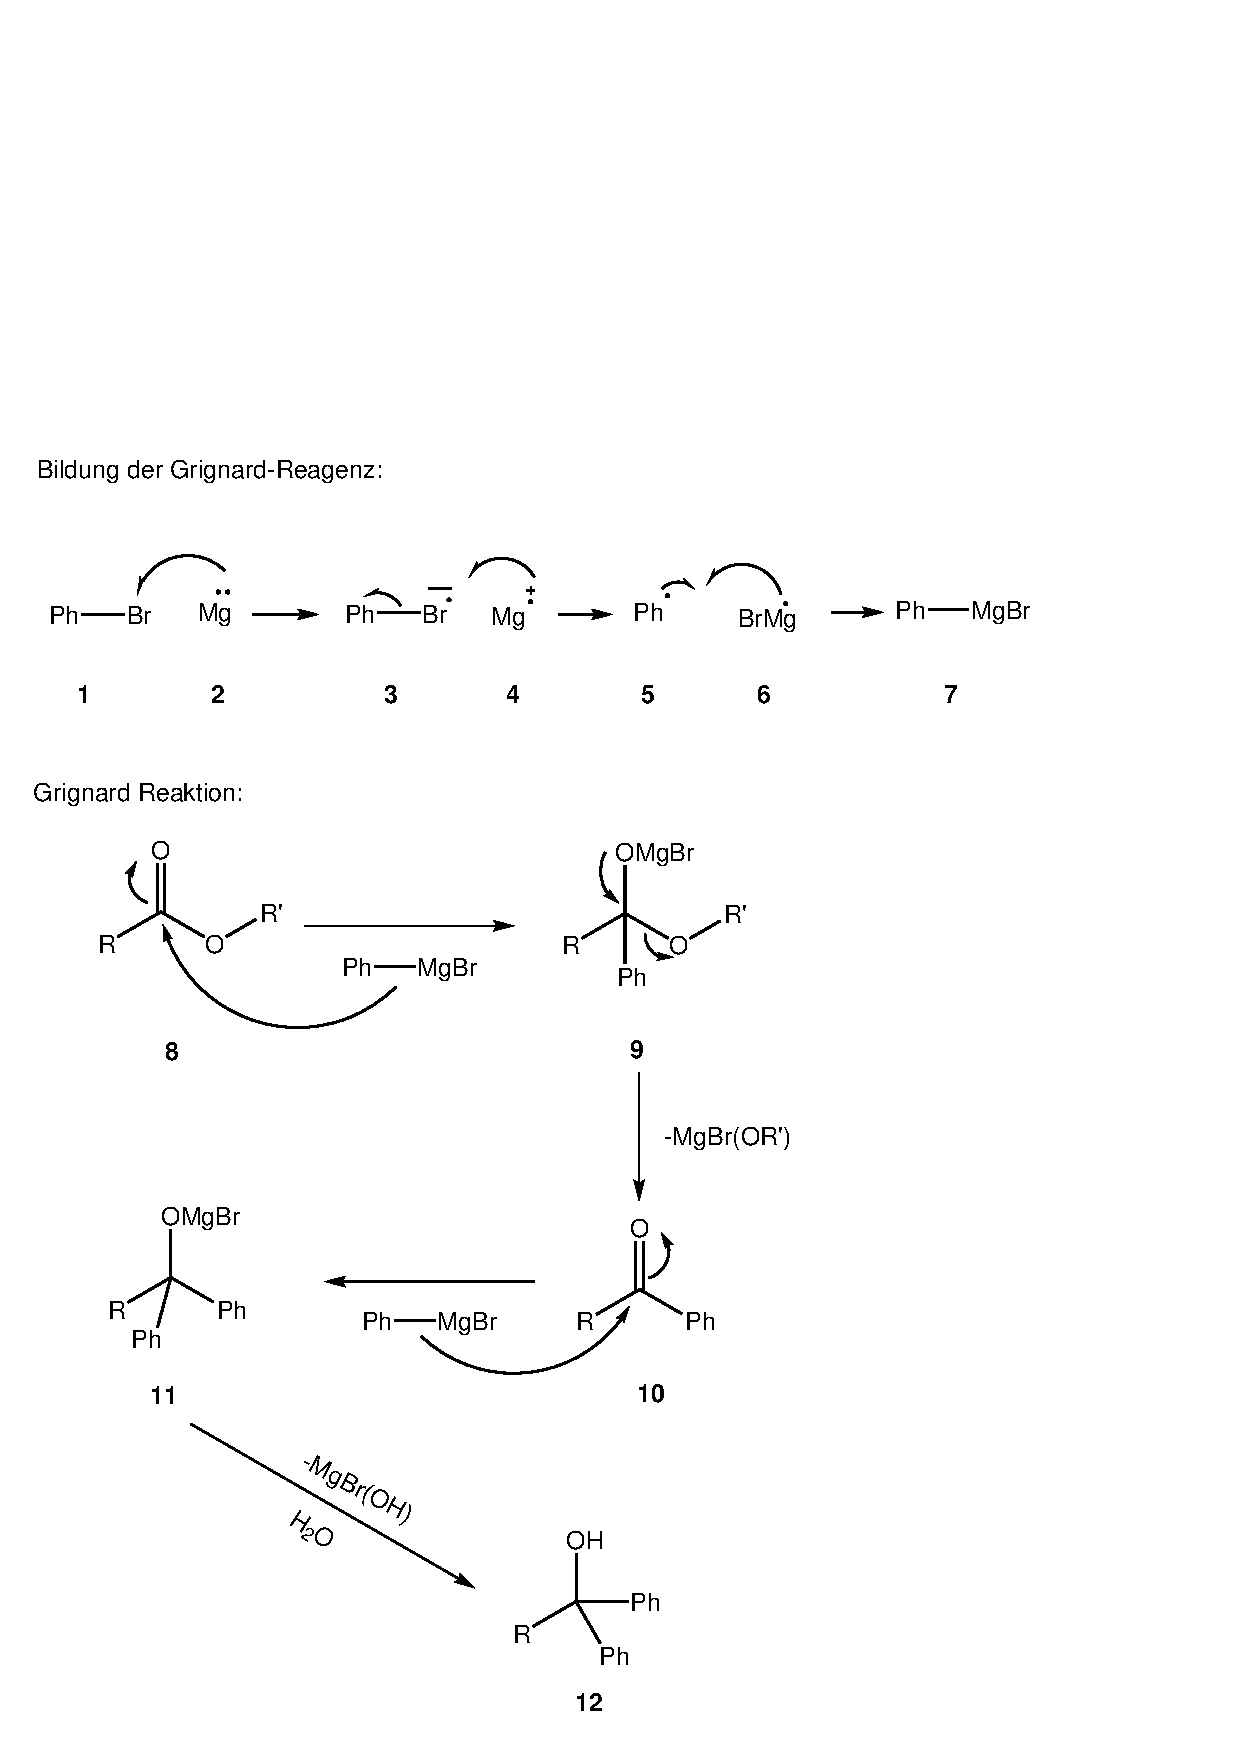
\includegraphics[width=\textwidth]{mechan.png}
\end{figure}
%\restoregeometry
\clearpage
\section{Abfallentsorgung}
Die nach dem Hydrolysieren verbleibenden wässrigen Phasen wurden
nach einer pH-Wertbestimmung im Behälter für basische wässrige Abfälle entsorgt.
Das im Rotationsverdampfer abgetrennte Lösungsmittel wurde im Behälter für halogenfreie Kohlenwasserstoffe entsorgt.
\section{Literatur}

\renewcommand{\section}[2]{}%
\def\bibindent{0em}
\begin{thebibliography}{99\kern\bibindent}
\makeatletter
\let\old@biblabel\@biblabel
\def\@biblabel#1{\old@biblabel{#1}\kern\bibindent}
\let\old@bibitem\bibitem
\def\bibitem#1{\old@bibitem{#1}\leavevmode\kern-\bibindent}
\makeatother
\bibitem{vor}
X. Gao, J. Han, L. Wang, \textit{Org. Letter.} \textbf{2015}, 4596 - 4599.
\bibitem{metall}
C. Elschenbroich, \textit{Organometallchemie}, 6. Aufl., Teubner, Wiesbaden \textbf{2005}, S. 64.
\bibitem{bio}
J. Buddrus, \textit{Grundlagen der Organische Chemie}, 4. Aufl., De Gruyter, Berlin \textbf{2011}, S. 496.
\end{thebibliography}
\end{onehalfspace}
\end{document}


